\section{Results}
\label{sec:results}

% Laptop and Mac measured so far; server and Raspberry Pi follow.

\paragraph{Generation.}
All 630 requests returned one code block without tool use. Claude Code answered fastest,
Antigravity CLI slowest (\cref{tab:gentime}); times include network latency.

\begin{table}[t]
  \centering
  \caption{Generation time per request in seconds ($n=210$ per LLM).}
  \label{tab:gentime}
  \footnotesize
  \begin{tabular}{@{}lrrrrr@{}}
    \toprule
    LLM & Mean & SD & Median & EB mean & CLBG mean \\
    \midrule
    Claude & 7.1  & 3.7  & 5.9  & 6.1  & 9.5  \\
    GPT    & 15.1 & 5.9  & 13.8 & 13.6 & 18.9 \\
    Gemini & 17.4 & 13.8 & 14.9 & 14.5 & 24.6 \\
    \bottomrule
  \end{tabular}
\end{table}

\paragraph{Measurements.}
Of 630 programs, 629 were correct on the laptop and 628 on the Mac, where one Java program printed decimals in the system's German locale.
Repetitions varied by 2.6\,\% (laptop) and 12\,\% (Mac; median coefficient of variation).
Generated Python consumed 11 (Mac: 16) times as much energy as C++ (geometric mean over
tasks), Java 2.5 (2.6) times (\cref{fig:languages}). Single algorithmic choices dominate the
LLM comparison (\cref{fig:llms}): Claude's C++ solutions for EB02 used 150--300 times
the others' energy. Relative to the task median, Gemini's programs used 0.90, GPT's 1.00,
and Claude's 1.29 on the laptop (Mac: 0.90, 1.01, 1.32). Program energies correlate across
platforms ($r=0.974$, log; \cref{fig:platforms}); energy and time correlate with
$r=0.997$ (laptop) and 0.963 (Mac).
\TODO{Server and Raspberry~Pi; mixed-effects models for RQ3/RQ4.}

\begin{figure}[t]
  \centering
  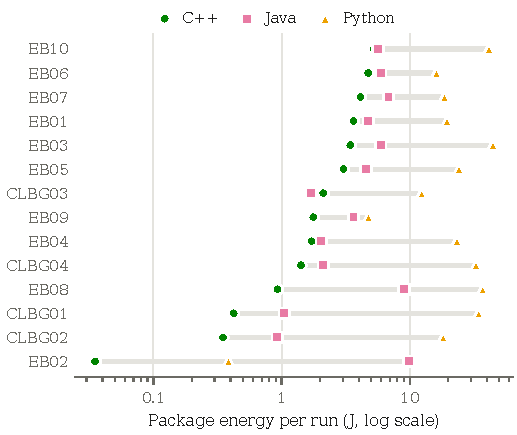
\includegraphics[width=\columnwidth]{laptop_languages}
  \caption{Median energy per run of generated programs (laptop).}
  \label{fig:languages}
\end{figure}

\begin{figure}[t]
  \centering
  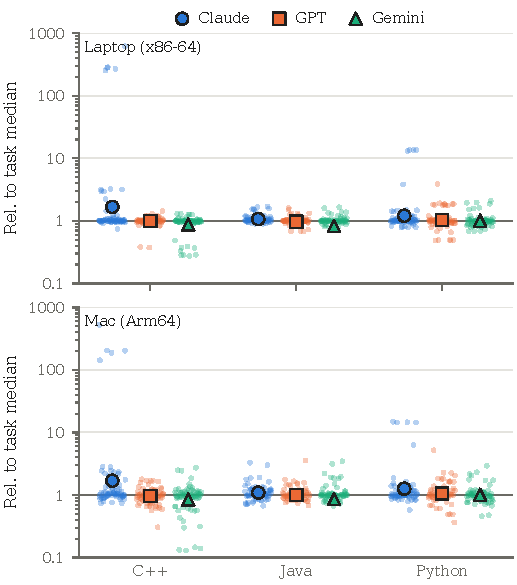
\includegraphics[width=\columnwidth]{llms}
  \caption{Program energy relative to its task--language median; large markers:
    geometric means.}
  \label{fig:llms}
\end{figure}

\begin{figure}[t]
  \centering
  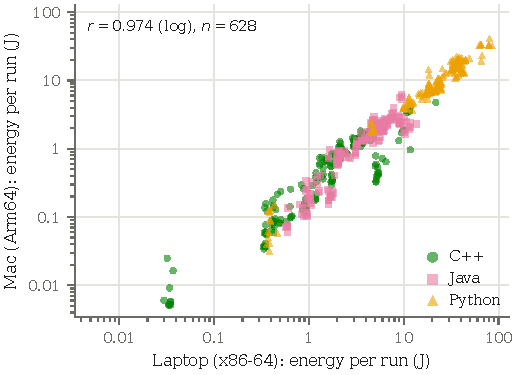
\includegraphics[width=\columnwidth]{platforms}
  \caption{Energy per program on laptop and Mac (different scopes).}
  \label{fig:platforms}
\end{figure}
